\documentclass[]{article}
\usepackage{lmodern}
\usepackage{amssymb,amsmath}
\usepackage{ifxetex,ifluatex}
\usepackage{fixltx2e} % provides \textsubscript
\ifnum 0\ifxetex 1\fi\ifluatex 1\fi=0 % if pdftex
  \usepackage[T1]{fontenc}
  \usepackage[utf8]{inputenc}
\else % if luatex or xelatex
  \ifxetex
    \usepackage{mathspec}
  \else
    \usepackage{fontspec}
  \fi
  \defaultfontfeatures{Ligatures=TeX,Scale=MatchLowercase}
\fi
% use upquote if available, for straight quotes in verbatim environments
\IfFileExists{upquote.sty}{\usepackage{upquote}}{}
% use microtype if available
\IfFileExists{microtype.sty}{%
\usepackage{microtype}
\UseMicrotypeSet[protrusion]{basicmath} % disable protrusion for tt fonts
}{}
\usepackage[margin=1in]{geometry}
\usepackage{hyperref}
\hypersetup{unicode=true,
            pdfborder={0 0 0},
            breaklinks=true}
\urlstyle{same}  % don't use monospace font for urls
\usepackage{color}
\usepackage{fancyvrb}
\newcommand{\VerbBar}{|}
\newcommand{\VERB}{\Verb[commandchars=\\\{\}]}
\DefineVerbatimEnvironment{Highlighting}{Verbatim}{commandchars=\\\{\}}
% Add ',fontsize=\small' for more characters per line
\usepackage{framed}
\definecolor{shadecolor}{RGB}{248,248,248}
\newenvironment{Shaded}{\begin{snugshade}}{\end{snugshade}}
\newcommand{\AlertTok}[1]{\textcolor[rgb]{0.94,0.16,0.16}{#1}}
\newcommand{\AnnotationTok}[1]{\textcolor[rgb]{0.56,0.35,0.01}{\textbf{\textit{#1}}}}
\newcommand{\AttributeTok}[1]{\textcolor[rgb]{0.77,0.63,0.00}{#1}}
\newcommand{\BaseNTok}[1]{\textcolor[rgb]{0.00,0.00,0.81}{#1}}
\newcommand{\BuiltInTok}[1]{#1}
\newcommand{\CharTok}[1]{\textcolor[rgb]{0.31,0.60,0.02}{#1}}
\newcommand{\CommentTok}[1]{\textcolor[rgb]{0.56,0.35,0.01}{\textit{#1}}}
\newcommand{\CommentVarTok}[1]{\textcolor[rgb]{0.56,0.35,0.01}{\textbf{\textit{#1}}}}
\newcommand{\ConstantTok}[1]{\textcolor[rgb]{0.00,0.00,0.00}{#1}}
\newcommand{\ControlFlowTok}[1]{\textcolor[rgb]{0.13,0.29,0.53}{\textbf{#1}}}
\newcommand{\DataTypeTok}[1]{\textcolor[rgb]{0.13,0.29,0.53}{#1}}
\newcommand{\DecValTok}[1]{\textcolor[rgb]{0.00,0.00,0.81}{#1}}
\newcommand{\DocumentationTok}[1]{\textcolor[rgb]{0.56,0.35,0.01}{\textbf{\textit{#1}}}}
\newcommand{\ErrorTok}[1]{\textcolor[rgb]{0.64,0.00,0.00}{\textbf{#1}}}
\newcommand{\ExtensionTok}[1]{#1}
\newcommand{\FloatTok}[1]{\textcolor[rgb]{0.00,0.00,0.81}{#1}}
\newcommand{\FunctionTok}[1]{\textcolor[rgb]{0.00,0.00,0.00}{#1}}
\newcommand{\ImportTok}[1]{#1}
\newcommand{\InformationTok}[1]{\textcolor[rgb]{0.56,0.35,0.01}{\textbf{\textit{#1}}}}
\newcommand{\KeywordTok}[1]{\textcolor[rgb]{0.13,0.29,0.53}{\textbf{#1}}}
\newcommand{\NormalTok}[1]{#1}
\newcommand{\OperatorTok}[1]{\textcolor[rgb]{0.81,0.36,0.00}{\textbf{#1}}}
\newcommand{\OtherTok}[1]{\textcolor[rgb]{0.56,0.35,0.01}{#1}}
\newcommand{\PreprocessorTok}[1]{\textcolor[rgb]{0.56,0.35,0.01}{\textit{#1}}}
\newcommand{\RegionMarkerTok}[1]{#1}
\newcommand{\SpecialCharTok}[1]{\textcolor[rgb]{0.00,0.00,0.00}{#1}}
\newcommand{\SpecialStringTok}[1]{\textcolor[rgb]{0.31,0.60,0.02}{#1}}
\newcommand{\StringTok}[1]{\textcolor[rgb]{0.31,0.60,0.02}{#1}}
\newcommand{\VariableTok}[1]{\textcolor[rgb]{0.00,0.00,0.00}{#1}}
\newcommand{\VerbatimStringTok}[1]{\textcolor[rgb]{0.31,0.60,0.02}{#1}}
\newcommand{\WarningTok}[1]{\textcolor[rgb]{0.56,0.35,0.01}{\textbf{\textit{#1}}}}
\usepackage{graphicx,grffile}
\makeatletter
\def\maxwidth{\ifdim\Gin@nat@width>\linewidth\linewidth\else\Gin@nat@width\fi}
\def\maxheight{\ifdim\Gin@nat@height>\textheight\textheight\else\Gin@nat@height\fi}
\makeatother
% Scale images if necessary, so that they will not overflow the page
% margins by default, and it is still possible to overwrite the defaults
% using explicit options in \includegraphics[width, height, ...]{}
\setkeys{Gin}{width=\maxwidth,height=\maxheight,keepaspectratio}
\IfFileExists{parskip.sty}{%
\usepackage{parskip}
}{% else
\setlength{\parindent}{0pt}
\setlength{\parskip}{6pt plus 2pt minus 1pt}
}
\setlength{\emergencystretch}{3em}  % prevent overfull lines
\providecommand{\tightlist}{%
  \setlength{\itemsep}{0pt}\setlength{\parskip}{0pt}}
\setcounter{secnumdepth}{0}
% Redefines (sub)paragraphs to behave more like sections
\ifx\paragraph\undefined\else
\let\oldparagraph\paragraph
\renewcommand{\paragraph}[1]{\oldparagraph{#1}\mbox{}}
\fi
\ifx\subparagraph\undefined\else
\let\oldsubparagraph\subparagraph
\renewcommand{\subparagraph}[1]{\oldsubparagraph{#1}\mbox{}}
\fi

%%% Use protect on footnotes to avoid problems with footnotes in titles
\let\rmarkdownfootnote\footnote%
\def\footnote{\protect\rmarkdownfootnote}

%%% Change title format to be more compact
\usepackage{titling}

% Create subtitle command for use in maketitle
\providecommand{\subtitle}[1]{
  \posttitle{
    \begin{center}\large#1\end{center}
    }
}

\setlength{\droptitle}{-2em}

  \title{}
    \pretitle{\vspace{\droptitle}}
  \posttitle{}
    \author{}
    \preauthor{}\postauthor{}
    \date{}
    \predate{}\postdate{}
  

\begin{document}

\hypertarget{brian-duran}{%
\subsubsection{Brian Durán}\label{brian-duran}}


\includegraphics{../logo_ciencia_de_datos.png}

Tarea: Sesión 4 y 5

\hypertarget{i-parte}{%
\paragraph{I Parte}\label{i-parte}}

\begin{enumerate}
\def\labelenumi{\arabic{enumi}.}
\tightlist
\item
  Sea \(P=(2,3)\), \(Q=(5,2)\), \(R=(2,-5)\) y \(S=(1,-2)\). Calcule
  \(proy_{\vec{PQ}}\vec{RS}\).
\end{enumerate}

\(\vec{PQ}\)

\begin{Shaded}
\begin{Highlighting}[]
\NormalTok{q <-}\StringTok{ }\KeywordTok{c}\NormalTok{(}\DecValTok{5}\NormalTok{,}\DecValTok{2}\NormalTok{)}
\NormalTok{p <-}\StringTok{ }\KeywordTok{c}\NormalTok{(}\DecValTok{2}\NormalTok{,}\DecValTok{3}\NormalTok{)}
\NormalTok{pq <-}\StringTok{ }\NormalTok{q }\OperatorTok{-}\StringTok{ }\NormalTok{p}
\NormalTok{pq}
\end{Highlighting}
\end{Shaded}

\begin{verbatim}
## [1]  3 -1
\end{verbatim}

\(\vec{RS}\)

\begin{Shaded}
\begin{Highlighting}[]
\NormalTok{r <-}\StringTok{ }\KeywordTok{c}\NormalTok{(}\DecValTok{2}\NormalTok{,}\OperatorTok{-}\DecValTok{5}\NormalTok{)}
\NormalTok{s <-}\StringTok{ }\KeywordTok{c}\NormalTok{(}\DecValTok{1}\NormalTok{,}\OperatorTok{-}\DecValTok{2}\NormalTok{)}
\NormalTok{rs <-}\StringTok{ }\NormalTok{s }\OperatorTok{-}\StringTok{ }\NormalTok{r}
\NormalTok{rs}
\end{Highlighting}
\end{Shaded}

\begin{verbatim}
## [1] -1  3
\end{verbatim}

\(proy_{\vec{PQ}}\vec{RS}\)

\begin{Shaded}
\begin{Highlighting}[]
\NormalTok{proy <-}\StringTok{ }\KeywordTok{project}\NormalTok{(rs, pq)}

\KeywordTok{fractions}\NormalTok{(proy)}
\end{Highlighting}
\end{Shaded}

\begin{verbatim}
## [1] -9/5  3/5
\end{verbatim}

\begin{enumerate}
\def\labelenumi{\arabic{enumi}.}
\setcounter{enumi}{1}
\tightlist
\item
  Sea \(u = (-2,1,6)\) y \(v = (2,4,5)\), comprueba que el vector \(w\)
  dado por \(w = u - \frac{u \cdot v}{\|v\|^2} v\) Es un vector
  ortogonal con \(v\)
\end{enumerate}

Calculamos:

\(u \cdot v\)

\begin{Shaded}
\begin{Highlighting}[]
\NormalTok{u <-}\StringTok{ }\KeywordTok{c}\NormalTok{(}\OperatorTok{-}\DecValTok{2}\NormalTok{,}\DecValTok{1}\NormalTok{,}\DecValTok{6}\NormalTok{)}
\NormalTok{v <-}\StringTok{ }\KeywordTok{c}\NormalTok{(}\DecValTok{2}\NormalTok{,}\DecValTok{4}\NormalTok{,}\DecValTok{5}\NormalTok{)}
\KeywordTok{sum}\NormalTok{(u}\OperatorTok{*}\NormalTok{v)}
\end{Highlighting}
\end{Shaded}

\begin{verbatim}
## [1] 30
\end{verbatim}

\({\|v\|^2}\)

\begin{Shaded}
\begin{Highlighting}[]
\NormalTok{v2 <-}\StringTok{ }\KeywordTok{norm}\NormalTok{(v, }\DataTypeTok{type=}\StringTok{"2"}\NormalTok{)}\OperatorTok{^}\DecValTok{2}
\NormalTok{v2}
\end{Highlighting}
\end{Shaded}

\begin{verbatim}
## [1] 45
\end{verbatim}

\(w = u - \frac{u \cdot v}{\|v\|^2} v\)

\begin{Shaded}
\begin{Highlighting}[]
\NormalTok{prod_punto_u_v =}\StringTok{ }\KeywordTok{sum}\NormalTok{(u}\OperatorTok{*}\NormalTok{v)}

\NormalTok{w =}\StringTok{ }\NormalTok{u }\OperatorTok{-}\StringTok{ }\NormalTok{((prod_punto_u_v }\OperatorTok{/}\StringTok{ }\NormalTok{v2) }\OperatorTok{*}\StringTok{ }\NormalTok{v)}

\NormalTok{w =}\StringTok{ }\KeywordTok{fractions}\NormalTok{(w)}

\KeywordTok{sum}\NormalTok{(w}\OperatorTok{*}\NormalTok{v)}
\end{Highlighting}
\end{Shaded}

\begin{verbatim}
## [1] 0
\end{verbatim}

\begin{Shaded}
\begin{Highlighting}[]
\KeywordTok{subspace}\NormalTok{(}\KeywordTok{as.matrix}\NormalTok{(w),}\KeywordTok{as.matrix}\NormalTok{(v))}
\end{Highlighting}
\end{Shaded}

\begin{verbatim}
## [1] 1.570796
\end{verbatim}

\begin{Shaded}
\begin{Highlighting}[]
\DecValTok{180}\OperatorTok{*}\KeywordTok{subspace}\NormalTok{(}\KeywordTok{as.matrix}\NormalTok{(w),}\KeywordTok{as.matrix}\NormalTok{(v))}\OperatorTok{/}\NormalTok{pi}
\end{Highlighting}
\end{Shaded}

\begin{verbatim}
## [1] 90
\end{verbatim}

\(W _{\bot } V ?\)

w es ortogonal con v, ya que la múltiplicación entre ellos es igual a
cero. Además de que el ángulo que los separa es igual a \(\pi\ /2\)

\begin{enumerate}
\def\labelenumi{\arabic{enumi}.}
\setcounter{enumi}{2}
\tightlist
\item
  Sean \(A=(3,0,0)\), \(B=(1,0,2)\), \(C=(2,3,0)\) puntos en el espacio
  (\(R^3\)).
\end{enumerate}

Con estos puntos:

\begin{enumerate}
\def\labelenumi{\alph{enumi}.}
\tightlist
\item
  Determine si el triángulo \(ABC\) es rectángulo, obtusángulo o
  acutángulo.
\end{enumerate}

\begin{Shaded}
\begin{Highlighting}[]
\NormalTok{a <-}\StringTok{ }\KeywordTok{c}\NormalTok{(}\DecValTok{3}\NormalTok{,}\DecValTok{0}\NormalTok{,}\DecValTok{0}\NormalTok{)}
\NormalTok{b <-}\StringTok{ }\KeywordTok{c}\NormalTok{(}\DecValTok{1}\NormalTok{,}\DecValTok{0}\NormalTok{,}\DecValTok{2}\NormalTok{)}
\NormalTok{c <-}\StringTok{ }\KeywordTok{c}\NormalTok{(}\DecValTok{2}\NormalTok{,}\DecValTok{3}\NormalTok{,}\DecValTok{0}\NormalTok{)}

\NormalTok{ab <-}\StringTok{ }\NormalTok{b}\OperatorTok{-}\NormalTok{a}
\NormalTok{bc <-}\StringTok{ }\NormalTok{c}\OperatorTok{-}\NormalTok{b}
\NormalTok{ca <-}\StringTok{ }\NormalTok{a}\OperatorTok{-}\NormalTok{c}

\DecValTok{180}\OperatorTok{*}\KeywordTok{subspace}\NormalTok{(}\KeywordTok{as.matrix}\NormalTok{(ab), }\KeywordTok{as.matrix}\NormalTok{(bc))}\OperatorTok{/}\NormalTok{pi}
\end{Highlighting}
\end{Shaded}

\begin{verbatim}
## [1] 55.46242
\end{verbatim}

\begin{Shaded}
\begin{Highlighting}[]
\DecValTok{180}\OperatorTok{*}\KeywordTok{subspace}\NormalTok{(}\KeywordTok{as.matrix}\NormalTok{(bc), }\KeywordTok{as.matrix}\NormalTok{(ca))}\OperatorTok{/}\NormalTok{pi}
\end{Highlighting}
\end{Shaded}

\begin{verbatim}
## [1] 47.45855
\end{verbatim}

\begin{Shaded}
\begin{Highlighting}[]
\DecValTok{180}\OperatorTok{*}\KeywordTok{subspace}\NormalTok{(}\KeywordTok{as.matrix}\NormalTok{(ab), }\KeywordTok{as.matrix}\NormalTok{(ca))}\OperatorTok{/}\NormalTok{pi}
\end{Highlighting}
\end{Shaded}

\begin{verbatim}
## [1] 77.07903
\end{verbatim}

Respuesta: El triángulo es acutángulo, ya que todos sus ángulos se
encuentran entre 0 y 90 grados.

\begin{enumerate}
\def\labelenumi{\alph{enumi}.}
\setcounter{enumi}{1}
\tightlist
\item
  Determine el perímetro del triángulo \(ABC\)
\end{enumerate}

\begin{Shaded}
\begin{Highlighting}[]
\NormalTok{norma_ab <-}\StringTok{ }\KeywordTok{norm}\NormalTok{(ab, }\DataTypeTok{type=}\StringTok{"2"}\NormalTok{)}
\NormalTok{norma_bc <-}\StringTok{ }\KeywordTok{norm}\NormalTok{(bc, }\DataTypeTok{type=}\StringTok{"2"}\NormalTok{)}
\NormalTok{norma_ca <-}\StringTok{ }\KeywordTok{norm}\NormalTok{(ca, }\DataTypeTok{type=}\StringTok{"2"}\NormalTok{)}

\NormalTok{perimetro <-}\StringTok{ }\NormalTok{norma_ab }\OperatorTok{+}\StringTok{ }\NormalTok{norma_bc }\OperatorTok{+}\StringTok{ }\NormalTok{norma_ca}
\NormalTok{perimetro}
\end{Highlighting}
\end{Shaded}

\begin{verbatim}
## [1] 9.732362
\end{verbatim}

\begin{enumerate}
\def\labelenumi{\alph{enumi}.}
\setcounter{enumi}{2}
\tightlist
\item
  Determine el área del triángulo ABC
\end{enumerate}

\begin{Shaded}
\begin{Highlighting}[]
\NormalTok{semiperimetro <-}\StringTok{ }\NormalTok{perimetro }\OperatorTok{/}\StringTok{ }\DecValTok{2}

\CommentTok{# Por formula de Héron}
\NormalTok{area =}\StringTok{ }\KeywordTok{sqrt}\NormalTok{(semiperimetro }\OperatorTok{*}\StringTok{ }\NormalTok{(semiperimetro }\OperatorTok{-}\StringTok{ }\NormalTok{norma_ab) }\OperatorTok{*}\StringTok{ }\NormalTok{(semiperimetro }\OperatorTok{-}\StringTok{ }\NormalTok{norma_bc) }\OperatorTok{*}\StringTok{ }\NormalTok{(semiperimetro }\OperatorTok{-}\StringTok{ }\NormalTok{norma_ca))}

\NormalTok{area}
\end{Highlighting}
\end{Shaded}

\begin{verbatim}
## [1] 4.358899
\end{verbatim}

\hypertarget{ii-parte}{%
\paragraph{II Parte}\label{ii-parte}}

\begin{enumerate}
\def\labelenumi{\arabic{enumi}.}
\tightlist
\item
  Compruebe que la matriz P, es ortogonal:
\end{enumerate}

\begin{Shaded}
\begin{Highlighting}[]
\NormalTok{p <-}\StringTok{ }\KeywordTok{matrix}\NormalTok{(}\KeywordTok{c}\NormalTok{(}\DecValTok{1}\OperatorTok{/}\DecValTok{2}\NormalTok{, }\DecValTok{1}\OperatorTok{/}\DecValTok{2}\NormalTok{, }\DecValTok{1}\OperatorTok{/}\DecValTok{2}\NormalTok{, }\DecValTok{1}\OperatorTok{/}\DecValTok{2}\NormalTok{, }
\NormalTok{              (}\DecValTok{1}\OperatorTok{/}\KeywordTok{sqrt}\NormalTok{(}\DecValTok{2}\NormalTok{)), }\OperatorTok{-}\NormalTok{(}\DecValTok{1}\OperatorTok{/}\KeywordTok{sqrt}\NormalTok{(}\DecValTok{2}\NormalTok{)), }\DecValTok{0}\NormalTok{, }\DecValTok{0}\NormalTok{, }
\NormalTok{              (}\DecValTok{1}\OperatorTok{/}\KeywordTok{sqrt}\NormalTok{(}\DecValTok{6}\NormalTok{)), (}\DecValTok{1}\OperatorTok{/}\KeywordTok{sqrt}\NormalTok{(}\DecValTok{6}\NormalTok{)), }\OperatorTok{-}\NormalTok{(}\DecValTok{2}\OperatorTok{/}\KeywordTok{sqrt}\NormalTok{(}\DecValTok{6}\NormalTok{)), }\DecValTok{0}\NormalTok{, }
\NormalTok{              (}\DecValTok{1}\OperatorTok{/}\NormalTok{(}\DecValTok{2}\OperatorTok{*}\KeywordTok{sqrt}\NormalTok{(}\DecValTok{3}\NormalTok{))), (}\DecValTok{1}\OperatorTok{/}\NormalTok{(}\DecValTok{2}\OperatorTok{*}\KeywordTok{sqrt}\NormalTok{(}\DecValTok{3}\NormalTok{))), (}\DecValTok{1}\OperatorTok{/}\NormalTok{(}\DecValTok{2}\OperatorTok{*}\KeywordTok{sqrt}\NormalTok{(}\DecValTok{3}\NormalTok{))), }\OperatorTok{-}\NormalTok{(}\DecValTok{3}\OperatorTok{/}\NormalTok{(}\DecValTok{2}\OperatorTok{*}\KeywordTok{sqrt}\NormalTok{(}\DecValTok{3}\NormalTok{)))), }
              \DataTypeTok{nrow=}\DecValTok{4}\NormalTok{, }\DataTypeTok{ncol=}\DecValTok{4}\NormalTok{, }\DataTypeTok{byrow=}\OtherTok{TRUE}\NormalTok{)}

\NormalTok{matriz_p <-}\StringTok{ }\KeywordTok{fractions}\NormalTok{(p)}

\NormalTok{matriz_p}
\end{Highlighting}
\end{Shaded}

\begin{verbatim}
##      [,1]           [,2]           [,3]           [,4]          
## [1,]            1/2            1/2            1/2            1/2
## [2,]      2378/3363     -5741/8119              0              0
## [3,]    19402/47525    19402/47525  -86329/105731              0
## [4,]   75658/262087   75658/262087   75658/262087 -489061/564719
\end{verbatim}

\begin{Shaded}
\begin{Highlighting}[]
\NormalTok{p_inversa <-}\StringTok{ }\KeywordTok{solve}\NormalTok{(matriz_p)}

\KeywordTok{fractions}\NormalTok{(p_inversa)}
\end{Highlighting}
\end{Shaded}

\begin{verbatim}
##      [,1]           [,2]           [,3]           [,4]          
## [1,]            1/2      2378/3363    19402/47525   75658/262087
## [2,]            1/2     -5741/8119    19402/47525   75658/262087
## [3,]            1/2              0  -86329/105731   75658/262087
## [4,]            1/2              0              0 -489061/564719
\end{verbatim}

\begin{Shaded}
\begin{Highlighting}[]
\NormalTok{p_transpuesta <-}\StringTok{ }\KeywordTok{t}\NormalTok{(p)}

\KeywordTok{fractions}\NormalTok{(p_transpuesta)}
\end{Highlighting}
\end{Shaded}

\begin{verbatim}
##      [,1]           [,2]           [,3]           [,4]          
## [1,]            1/2      2378/3363    19402/47525   75658/262087
## [2,]            1/2     -5741/8119    19402/47525   75658/262087
## [3,]            1/2              0  -86329/105731   75658/262087
## [4,]            1/2              0              0 -489061/564719
\end{verbatim}

La matriz P es ortogonal puesto que su inversa y su transpuesta son
iguales.

\begin{enumerate}
\def\labelenumi{\arabic{enumi}.}
\setcounter{enumi}{1}
\tightlist
\item
  Demuestre que A es indempotente.
\end{enumerate}

\begin{Shaded}
\begin{Highlighting}[]
\NormalTok{a <-}\StringTok{ }\KeywordTok{matrix}\NormalTok{(}\KeywordTok{c}\NormalTok{(}\DecValTok{2}\NormalTok{, }\DecValTok{-2}\NormalTok{, }\DecValTok{-4}\NormalTok{, }
              \DecValTok{-1}\NormalTok{, }\DecValTok{3}\NormalTok{, }\DecValTok{4}\NormalTok{,}
              \DecValTok{1}\NormalTok{, }\DecValTok{-2}\NormalTok{, }\DecValTok{-3}\NormalTok{), }
              \DecValTok{3}\NormalTok{, }\DecValTok{3}\NormalTok{, }\DataTypeTok{byrow=}\OtherTok{TRUE}\NormalTok{)}


\NormalTok{a}
\end{Highlighting}
\end{Shaded}

\begin{verbatim}
##      [,1] [,2] [,3]
## [1,]    2   -2   -4
## [2,]   -1    3    4
## [3,]    1   -2   -3
\end{verbatim}

\begin{Shaded}
\begin{Highlighting}[]
\NormalTok{a}\OperatorTok\NormalTok{a}
\end{Highlighting}
\end{Shaded}

\begin{verbatim}
##      [,1] [,2] [,3]
## [1,]    2   -2   -4
## [2,]   -1    3    4
## [3,]    1   -2   -3
\end{verbatim}

La matriz A es idempotente puesto que es igual a ella misma al cuadrado.

\begin{enumerate}
\def\labelenumi{\arabic{enumi}.}
\setcounter{enumi}{2}
\tightlist
\item
  Determine la composición \(f(m)\)
\end{enumerate}

\begin{Shaded}
\begin{Highlighting}[]
\NormalTok{m <-}\StringTok{ }\KeywordTok{matrix}\NormalTok{(}\KeywordTok{c}\NormalTok{(}\DecValTok{3}\OperatorTok{/}\DecValTok{2}\NormalTok{, }\DecValTok{-5}\OperatorTok{/}\DecValTok{2}\NormalTok{, }
              \DecValTok{2}\OperatorTok{/}\DecValTok{3}\NormalTok{, }\DecValTok{-1}\OperatorTok{/}\DecValTok{3}\NormalTok{), }
              \DecValTok{2}\NormalTok{, }\DecValTok{2}\NormalTok{, }\DataTypeTok{byrow=}\OtherTok{TRUE}\NormalTok{)}

\KeywordTok{fractions}\NormalTok{(m)}
\end{Highlighting}
\end{Shaded}

\begin{verbatim}
##      [,1] [,2]
## [1,]  3/2 -5/2
## [2,]  2/3 -1/3
\end{verbatim}

\begin{Shaded}
\begin{Highlighting}[]
\NormalTok{m3 <-}\StringTok{ }\NormalTok{m}\OperatorTok\NormalTok{m}\OperatorTok\NormalTok{m}

\NormalTok{m2 <-}\StringTok{ }\NormalTok{m}\OperatorTok\NormalTok{m}

\NormalTok{fx =}\StringTok{ }\DecValTok{6}\OperatorTok{*}\NormalTok{m3 }\OperatorTok{+}\StringTok{ }\DecValTok{3}\OperatorTok{*}\NormalTok{m2 }\OperatorTok{-}\StringTok{ }\NormalTok{m}

\KeywordTok{fractions}\NormalTok{(fx)}
\end{Highlighting}
\end{Shaded}

\begin{verbatim}
##      [,1]   [,2]  
## [1,]  -37/6  -55/6
## [2,]   22/9 -116/9
\end{verbatim}

\begin{enumerate}
\def\labelenumi{\arabic{enumi}.}
\setcounter{enumi}{3}
\tightlist
\item
  Encuentre la matriz inversa y el determinante de cada una de las
  siguientes matrices:
\end{enumerate}

\begin{Shaded}
\begin{Highlighting}[]
\NormalTok{a <-}\StringTok{ }\KeywordTok{matrix}\NormalTok{(}\KeywordTok{c}\NormalTok{(}\DecValTok{1}\NormalTok{, }\DecValTok{2}\NormalTok{, }\DecValTok{3}\NormalTok{, }
              \DecValTok{2}\NormalTok{, }\DecValTok{5}\NormalTok{, }\DecValTok{7}\NormalTok{,}
              \DecValTok{-2}\NormalTok{, }\DecValTok{-4}\NormalTok{, }\DecValTok{-5}\NormalTok{), }
              \DecValTok{3}\NormalTok{, }\DecValTok{3}\NormalTok{, }\DataTypeTok{byrow=}\OtherTok{TRUE}\NormalTok{)}

\KeywordTok{solve}\NormalTok{(a)}
\end{Highlighting}
\end{Shaded}

\begin{verbatim}
##      [,1] [,2] [,3]
## [1,]    3   -2   -1
## [2,]   -4    1   -1
## [3,]    2    0    1
\end{verbatim}

\begin{Shaded}
\begin{Highlighting}[]
\KeywordTok{det}\NormalTok{(a)}
\end{Highlighting}
\end{Shaded}

\begin{verbatim}
## [1] 1
\end{verbatim}

\begin{Shaded}
\begin{Highlighting}[]
\NormalTok{b <-}\StringTok{ }\KeywordTok{matrix}\NormalTok{(}\KeywordTok{c}\NormalTok{(}\DecValTok{3}\NormalTok{, }\DecValTok{-2}\NormalTok{, }\DecValTok{-1}\NormalTok{, }
              \DecValTok{-4}\NormalTok{, }\DecValTok{1}\NormalTok{, }\DecValTok{-1}\NormalTok{,}
              \DecValTok{2}\NormalTok{, }\DecValTok{0}\NormalTok{, }\DecValTok{1}\NormalTok{), }
              \DecValTok{3}\NormalTok{, }\DecValTok{3}\NormalTok{, }\DataTypeTok{byrow=}\OtherTok{TRUE}\NormalTok{)}

\KeywordTok{solve}\NormalTok{(b)}
\end{Highlighting}
\end{Shaded}

\begin{verbatim}
##      [,1] [,2] [,3]
## [1,]    1    2    3
## [2,]    2    5    7
## [3,]   -2   -4   -5
\end{verbatim}

\begin{Shaded}
\begin{Highlighting}[]
\KeywordTok{det}\NormalTok{(b)}
\end{Highlighting}
\end{Shaded}

\begin{verbatim}
## [1] 1
\end{verbatim}

\begin{Shaded}
\begin{Highlighting}[]
\NormalTok{c <-}\StringTok{ }\KeywordTok{matrix}\NormalTok{(}\KeywordTok{c}\NormalTok{(}\DecValTok{0}\NormalTok{, }\DecValTok{2}\NormalTok{, }\DecValTok{1}\NormalTok{, }
              \DecValTok{1}\NormalTok{, }\DecValTok{3}\NormalTok{, }\DecValTok{-1}\NormalTok{,}
              \DecValTok{-1}\NormalTok{, }\DecValTok{1}\NormalTok{, }\DecValTok{2}\NormalTok{), }
              \DecValTok{3}\NormalTok{, }\DecValTok{3}\NormalTok{, }\DataTypeTok{byrow=}\OtherTok{TRUE}\NormalTok{)}

\KeywordTok{fractions}\NormalTok{(}\KeywordTok{solve}\NormalTok{(c))}
\end{Highlighting}
\end{Shaded}

\begin{verbatim}
##      [,1] [,2] [,3]
## [1,]  7/2 -3/2 -5/2
## [2,] -1/2  1/2  1/2
## [3,]    2   -1   -1
\end{verbatim}

\begin{Shaded}
\begin{Highlighting}[]
\KeywordTok{det}\NormalTok{(c)}
\end{Highlighting}
\end{Shaded}

\begin{verbatim}
## [1] 2
\end{verbatim}

\begin{Shaded}
\begin{Highlighting}[]
\NormalTok{d <-}\StringTok{ }\KeywordTok{matrix}\NormalTok{(}\KeywordTok{c}\NormalTok{(}\DecValTok{3}\NormalTok{, }\DecValTok{6}\NormalTok{, }\DecValTok{9}\NormalTok{, }
              \DecValTok{2}\NormalTok{, }\DecValTok{5}\NormalTok{, }\DecValTok{1}\NormalTok{,}
              \DecValTok{1}\NormalTok{, }\DecValTok{1}\NormalTok{, }\DecValTok{8}\NormalTok{), }
              \DecValTok{3}\NormalTok{, }\DecValTok{3}\NormalTok{, }\DataTypeTok{byrow=}\OtherTok{TRUE}\NormalTok{)}

\KeywordTok{det}\NormalTok{(d)}
\end{Highlighting}
\end{Shaded}

\begin{verbatim}
## [1] 0
\end{verbatim}

La última matriz no tiene inversa puesto que el determinante es cero, es
decir la matriz es singular o invertible.

Que relación existe entre las matrices que poseen inversas y el valor de
su determinante? Sug: revisar la teoría vista en clase. Cuando una
matriz posee inversa, se puede asumir que su determinante es mayor a
cero.

\begin{enumerate}
\def\labelenumi{\arabic{enumi}.}
\setcounter{enumi}{4}
\tightlist
\item
  ¿Cómo se propaga una enfermedad contagiosa?. Suponga que un grupo de 4
  individuos que llamaremos \(I_{1}, I_{2}, I_{3}, I_{4}\), han
  contraído una enfermedad.
\end{enumerate}

Este grupo entra en contacto con 6 personas de un segundo grupo:
\(P_{1}, P_{2}, P_{3}, P_{4}, P_{5}, P_{6}\). Este tipo de contactos se
llaman directos y se pueden representar en una matriz de 4 x 6, como la
que se muestra a continuación:

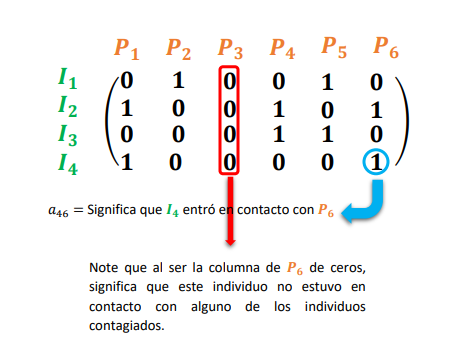
\includegraphics{matriz_contagio.png}

Note que la forma de construir dicha matriz es, colocando un 1 si una
persona del primer grupo (contagiados) entra en contacto con alguna
persona del segundo grupo.

Llamemos \(A\) a esta matriz de contactos Primer Contacto Directo:

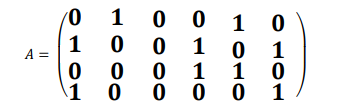
\includegraphics{matriz_a.png}

Ahora suponga que las 6 personas del grupo 2 entró en contacto directo
con un tercer grupo de cinco personas
\(M_{1}, M_{2}, M_{3}, M_{4}, M_{5}, M_{6}\) de la siguiente manera:

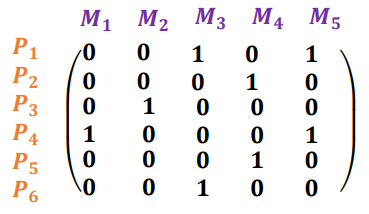
\includegraphics{matriz_contagio_indirecto.png}

Llamamos \(B\) a esta segunda matriz de contacto:

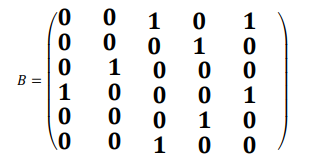
\includegraphics{matriz_b.png}

La lógica es igual que en el caso anterior, 1 significa que un individuo
del segundo grupo estuvo en contacto con un individuo del tercer grupo.
Los contactos indirectos o de segundo orden, se pueden dar entre
individuos del primer grupo con individuos del tercer grupo, esto es,
que una persona del grupo 3, puede ser contagiada por alguien del grupo
2 que a su vez fue contagiada por alguien del grupo 1. A manera de
ejemplo, note que las posiciones \(a_{24}=1\ y \ b_{45}=1\), con esto,
se ve que indirectamente la quinta persona del grupo 3, tuvo contacto
con una persona del grupo 1 a través de la cuarta persona del grupo 2,
así:

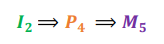
\includegraphics{arrows.png}

Con respecto al caso anterior, realice los siguiente:

\begin{enumerate}
\def\labelenumi{\alph{enumi}.}
\tightlist
\item
  Calcule una nueva matriz \(C\), tal que \(C=A \cdot B\) (Tome en
  cuenta que el producto es matricial, al trabajarlo en R).
\end{enumerate}

\begin{Shaded}
\begin{Highlighting}[]
\NormalTok{a_encabezados =}\StringTok{ }\KeywordTok{list}\NormalTok{(}\KeywordTok{c}\NormalTok{(}\StringTok{"I1"}\NormalTok{, }\StringTok{"I2"}\NormalTok{, }\StringTok{"I3"}\NormalTok{, }\StringTok{"I4"}\NormalTok{), }\KeywordTok{c}\NormalTok{(}\StringTok{"P1"}\NormalTok{, }\StringTok{"P2"}\NormalTok{, }\StringTok{"P3"}\NormalTok{, }\StringTok{"P4"}\NormalTok{, }\StringTok{"P5"}\NormalTok{, }\StringTok{"P6"}\NormalTok{))}

\NormalTok{a <-}\StringTok{ }\KeywordTok{matrix}\NormalTok{(}\KeywordTok{c}\NormalTok{(}\DecValTok{0}\NormalTok{, }\DecValTok{1}\NormalTok{, }\DecValTok{0}\NormalTok{, }\DecValTok{0}\NormalTok{, }\DecValTok{1}\NormalTok{, }\DecValTok{0}\NormalTok{,}
              \DecValTok{1}\NormalTok{, }\DecValTok{0}\NormalTok{, }\DecValTok{0}\NormalTok{, }\DecValTok{1}\NormalTok{, }\DecValTok{0}\NormalTok{, }\DecValTok{1}\NormalTok{,}
              \DecValTok{0}\NormalTok{, }\DecValTok{0}\NormalTok{, }\DecValTok{0}\NormalTok{, }\DecValTok{1}\NormalTok{, }\DecValTok{1}\NormalTok{, }\DecValTok{0}\NormalTok{,}
              \DecValTok{1}\NormalTok{, }\DecValTok{0}\NormalTok{, }\DecValTok{0}\NormalTok{, }\DecValTok{0}\NormalTok{, }\DecValTok{0}\NormalTok{, }\DecValTok{1}\NormalTok{),}
              \DecValTok{4}\NormalTok{, }\DecValTok{6}\NormalTok{, }\DataTypeTok{byrow=}\OtherTok{TRUE}\NormalTok{, }\DataTypeTok{dimnames=}\NormalTok{a_encabezados)}

\NormalTok{a}
\end{Highlighting}
\end{Shaded}

\begin{verbatim}
##    P1 P2 P3 P4 P5 P6
## I1  0  1  0  0  1  0
## I2  1  0  0  1  0  1
## I3  0  0  0  1  1  0
## I4  1  0  0  0  0  1
\end{verbatim}

\begin{Shaded}
\begin{Highlighting}[]
\NormalTok{b_encabezados =}\StringTok{ }\KeywordTok{list}\NormalTok{(}\KeywordTok{c}\NormalTok{(}\StringTok{"P1"}\NormalTok{, }\StringTok{"P2"}\NormalTok{, }\StringTok{"P3"}\NormalTok{, }\StringTok{"P4"}\NormalTok{, }\StringTok{"P5"}\NormalTok{, }\StringTok{"P6"}\NormalTok{), }\KeywordTok{c}\NormalTok{(}\StringTok{"M1"}\NormalTok{, }\StringTok{"M2"}\NormalTok{, }\StringTok{"M3"}\NormalTok{, }\StringTok{"M4"}\NormalTok{, }\StringTok{"M5"}\NormalTok{))}

\NormalTok{b <-}\StringTok{ }\KeywordTok{matrix}\NormalTok{(}\KeywordTok{c}\NormalTok{(}\DecValTok{0}\NormalTok{, }\DecValTok{0}\NormalTok{, }\DecValTok{1}\NormalTok{, }\DecValTok{0}\NormalTok{, }\DecValTok{1}\NormalTok{,}
              \DecValTok{0}\NormalTok{, }\DecValTok{0}\NormalTok{, }\DecValTok{0}\NormalTok{, }\DecValTok{1}\NormalTok{, }\DecValTok{0}\NormalTok{,}
              \DecValTok{0}\NormalTok{, }\DecValTok{1}\NormalTok{, }\DecValTok{0}\NormalTok{, }\DecValTok{0}\NormalTok{, }\DecValTok{0}\NormalTok{,}
              \DecValTok{1}\NormalTok{, }\DecValTok{0}\NormalTok{, }\DecValTok{0}\NormalTok{, }\DecValTok{0}\NormalTok{, }\DecValTok{1}\NormalTok{,}
              \DecValTok{0}\NormalTok{, }\DecValTok{0}\NormalTok{, }\DecValTok{0}\NormalTok{, }\DecValTok{1}\NormalTok{, }\DecValTok{0}\NormalTok{,}
              \DecValTok{0}\NormalTok{, }\DecValTok{0}\NormalTok{, }\DecValTok{1}\NormalTok{, }\DecValTok{0}\NormalTok{, }\DecValTok{0}\NormalTok{),}
              \DecValTok{6}\NormalTok{, }\DecValTok{5}\NormalTok{, }\DataTypeTok{byrow=}\OtherTok{TRUE}\NormalTok{, }\DataTypeTok{dimnames=}\NormalTok{b_encabezados)}
\NormalTok{b}
\end{Highlighting}
\end{Shaded}

\begin{verbatim}
##    M1 M2 M3 M4 M5
## P1  0  0  1  0  1
## P2  0  0  0  1  0
## P3  0  1  0  0  0
## P4  1  0  0  0  1
## P5  0  0  0  1  0
## P6  0  0  1  0  0
\end{verbatim}

\begin{Shaded}
\begin{Highlighting}[]
\NormalTok{c <-}\StringTok{ }\NormalTok{a}\OperatorTok\NormalTok{b}
\NormalTok{c}
\end{Highlighting}
\end{Shaded}

\begin{verbatim}
##    M1 M2 M3 M4 M5
## I1  0  0  0  2  0
## I2  1  0  2  0  2
## I3  1  0  0  1  1
## I4  0  0  2  0  1
\end{verbatim}

\begin{enumerate}
\def\labelenumi{\alph{enumi}.}
\setcounter{enumi}{1}
\tightlist
\item
  ¿Cuáles grupos de individuos (Grupo 1, 2 o 3) están quedando
  representados en \(C\)?, ¿quiénes están representados en las filas y
  quiénes en las columnas?
\end{enumerate}

En la matriz \(C\) se están representanto los individuos de los tres
grupos, ya que se demuestran los contactos directos e indirectos. Las
filas representan a los individuos del grupo 1 (\(I\)) y la sumatoria de
la fila representa los contactos indirectos que tuvo el individuo
\(I_n\) con miembros del grupo \(M\) a través de miembros del grupo
\(P\). Las columnas representan a los miembros del grupo 3 (\(M\)) y la
sumatoria de la columna la cantidad total de contactos indirectos que
tuvo el individuo (\(M_n\)) con individuos del grupo \(I\) a través de
\(P\).

\begin{enumerate}
\def\labelenumi{\alph{enumi}.}
\setcounter{enumi}{2}
\tightlist
\item
  Tome la fila 2 de \(C\) e interprétela (haga la extracción de esta
  usando un comando apropiado en R).
\end{enumerate}

\begin{Shaded}
\begin{Highlighting}[]
\NormalTok{c[}\DecValTok{2}\NormalTok{,]}
\end{Highlighting}
\end{Shaded}

\begin{verbatim}
## M1 M2 M3 M4 M5 
##  1  0  2  0  2
\end{verbatim}

El individuo \(I_{2}\) fue la persona que más contagio a miembros del
grupo \(M\) de manera indirecta.

\begin{enumerate}
\def\labelenumi{\alph{enumi}.}
\setcounter{enumi}{3}
\tightlist
\item
  Tome la columna 2 y 5 de \(C\) e interprételas (Use comandos
  apropiados en R para la extracción)
\end{enumerate}

\begin{Shaded}
\begin{Highlighting}[]
\NormalTok{c[,}\DecValTok{2}\NormalTok{]}
\end{Highlighting}
\end{Shaded}

\begin{verbatim}
## I1 I2 I3 I4 
##  0  0  0  0
\end{verbatim}

El individuo \(M_{2}\) no tuvo contacto con algún \(P\) que tuviera
contacto con algún \(I\). Por lo tanto \(M_{2}\) no fue contagiado.

\begin{Shaded}
\begin{Highlighting}[]
\NormalTok{c[,}\DecValTok{5}\NormalTok{]}
\end{Highlighting}
\end{Shaded}

\begin{verbatim}
## I1 I2 I3 I4 
##  0  2  1  1
\end{verbatim}

El individuo \(M_{5}\) fue el miembro del grupo 3 que más contactos
indirectos tuvo con miembros del grupo 1 \(I\).

\begin{enumerate}
\def\labelenumi{\alph{enumi}.}
\setcounter{enumi}{4}
\tightlist
\item
  Interprete la posición \(C_{43}\) (Extraiga la entrada, usando el
  comando apropiado en R).
\end{enumerate}

\begin{Shaded}
\begin{Highlighting}[]
\NormalTok{c[}\DecValTok{4}\NormalTok{,}\DecValTok{3}\NormalTok{]}
\end{Highlighting}
\end{Shaded}

\begin{verbatim}
## [1] 2
\end{verbatim}

El individuo \(I_4\) tuvo \textbf{2} contactos indirectos con el miembro
\(M_3\) a través de 2 miembros del grupo 2 (\(P\))

~

Autor Brian Duran

{\href{mailto:bduran0393@gmail.com}{\nolinkurl{bduran0393@gmail.com}}}

~


\end{document}
